%% This is emulateapj reformatting of the AASTEX sample document
%%
\documentclass[iop]{emulateapj}

\newcommand{\vdag}{(v)^\dagger}
\newcommand{\myemail}{skywalker@galaxy.far.far.away}

%% You can insert a short comment on the title page using the command below.



%% If you wish, you may supply running head information, although
%% this information may be modified by the editorial offices.
%% The left head contains a list of authors,
%% usually a maximum of three (otherwise use et al.).  The right
%% head is a modified title of up to roughly 44 characters.
%% Running heads will not print in the manuscript style.

\shorttitle{Kinematic Evolution}
\shortauthors{Tyler Baines}

%% This is the end of the preamble.  Indicate the beginning of the
%% paper itself with \begin{document}.

\begin{document}

%% LaTeX will automatically break titles if they run longer than
%% one line. However, you may use \\ to force a line break if
%% you desire.

\title{Evolution of the Kinematics of MW/M31 Bulges during and after the Merger}

%% Use \author, \affil, and the \and command to format
%% author and affiliation information.
%% Note that \email has replaced the old \authoremail command
%% from AASTeX v4.0. You can use \email to mark an email address
%% anywhere in the paper, not just in the front matter.
%% As in the title, use \\ to force line breaks.

\author{Tyler Baines}


%% Notice that each of these authors has alternate affiliations, which
%% are identified by the \altaffilmark after each name.  Specify alternate
%% affiliation information with \altaffiltext, with one command per each
%% affiliation.

%% Mark off your abstract in the ``abstract'' environment. In the manuscript
%% style, abstract will output a Received/Accepted line after the
%% title and affiliation information. No date will appear since the author
%% does not have this information. The dates will be filled in by the
%% editorial office after submission.

\begin{abstract}
Understanding the fundamental evolution in dynamical processes during mergers is a key to comprehend galactic evolution. In this paper we study the kinematic evolution of the bulge components and the dynamical stability of Remnant of the MW-M31-M33 system by analyzing \textit{N}-Body simulation data. The bulge component is embedded in the inner most regions of a galaxy which becomes difficult to study due to the disk components with respect to its orientation due to our line of sight. We find the system it self is dynamically stable but a high mass concentration is found at radii $r<5$ kpc but is still supported by the Virial Profiles. The Bulge supports a skewed gaussian distribution with a dispersion value of $\sigma=111.72$ km s$^{-1}$. A Sersic Profile with a sersic index of $n=4$ resulting in a classical bulge feature . The evolution of the bulge during the merger result in similar line profiles to that of the MW and M31. 

\end{abstract}

%% Keywords should appear after the \end{abstract} command. The uncommented
%% example has been keyed in ApJ style. See the instructions to authors
%% for the journal to which you are submitting your paper to determine
%% what keyword punctuation is appropriate.

%% Authors who wish to have the most important objects in their paper
%% linked in the electronic edition to a data center may do so in the
%% subject header.  Objects should be in the appropriate "individual"
%% headers (e.g. quasars: individual, stars: individual, etc.) with the
%% additional provision that the total number of headers, including each
%% individual object, not exceed six.  The \objectname{} macro, and its
%% alias \object{}, is used to mark each object.  The macro takes the object
%% name as its primary argument.  This name will appear in the paper
%% and serve as the link's anchor in the electronic edition if the name
%% is recognized by the data centers.  The macro also takes an optional
%% argument in parentheses in cases where the data center identification
%% differs from what is to be printed in the paper.

\keywords{galactic evolution: mergers ---
local group: \objectname{MW},
\object{M31}, \objectname{M33}}

%% From the front matter, we move on to the body of the paper.
%% In the first two sections, notice the use of the natbib \citep
%% and \citet commands to identify citations.  The citations are
%% tied to the reference list via symbolic KEYs. The KEY corresponds
%% to the KEY in the \bibitem in the reference list below. We have
%% chosen the first three characters of the first author's name plus
%% the last two numeral of the year of publication as our KEY for
%% each reference.

\section{Introduction}
It is is still unclear whether merger events between two disk galaxies result in an elliptical type. Using cosmic simulation helps us observed and understand the underlining physics of galaxy-galaxy interactions over long time scales. And using these simulations we can compare them to observations and test whether our theories hold true. \citep{zepf1997formation} suggests two process in which ellipticals form either through mergers or due to star formation burst surrounded by dust.  The more highly recognized scenario is that ellipticals form from mergers which \citep{kormendy2009structure} verifies, and \citep{querejeta2015formation} conclude that merger events of spirals result in S0 types. Although the process whether how galaxies form and evolve over is still open for debate. But observations allow to through still the components that make up typical disk galaxies such as the Milky Way (MW from no own) and Messier 31 (M31 from now on). Studying the disk and halo components reside in the outer regions of the galaxies which make them rather easier to observe. The inner regions where bulges however located in the central regions are obscured by dust and gas blocking light base of the orientation of the galaxy to our line of sight make it difficult to do in-depth studies. This is where cosmic simulations can allow us to study the bulge indirectly. The bulge of a galaxy is either classified as a classical or a puesdobulge base on its morphology pertaining to spherically symmetric or asymmetric (boxy or peanut shaped). Classical Bulges have properties of spherical symmetry that are dispersion support, which can also be fitted to Sersic Profiles with Sersic indices $n\geq2$ while psuedobulges have $n<2$. Understanding how the bulge growth and dynamics changes overtime and through mergers can impact our understanding of galactic evolution and the formation of early-type galaxies or that the bulge are the sole responsibility why we observe these galaxies.






\section{This Project}
For this project I will be exploring the kinematics and mass distributions of the MW-M31 Merger to analyze how the internal component, the bulge, of the system is effected during and after the merger and test for dynamical stability.  Since the bulge lies in the center, the gravitational potential is much stronger compared to the other components. This could mean that bulges should undergo the least amount of change compared to its counter parts. But results may vary depending on overall size and mass of the two colliding galaxy. We know from simulations that mergers are violent interactions that change the galaxies morphology each encounter resulting in instability. It is worth investigating how the bulge components are effected and verify is the inner regions to show stability or not. 



\section{Methods}
\subsection{\textit{N}-Body Simulation}
A collisionless \textit{N}-body simulation was used to explore the MW-M31-M33 system. Various intital conditions were chosen for the galaxies. The disk an bulge component intial condition were selected based off the literature, while the halos are given by Hernquirst profiles. This simulation excluded the effects of gas, allowing high quality data to be obtained, and starts at todays time and intergrate forward in time $\tau<12$ Gyr. \citep{van2012m31}

\subsection{My Code}
For this paper, I developed a code that finds the snapshot file pertaining to a specific time that one may want to analyzed. I also wrote code to generate various line profiles to test Virial Stability. To do so we adopted the Virial Theorem and Jean's Equations to test whether the remnant's bulge meets these conditions. Also a modified Sersic Profile that required five initial parameters. 	










\section{Results}
In order to analyze the evolution of the bulge component particles four distinct snapshots: 0, 335, 424, 721. These snapshots correspond to times: 0, 4.79, 6.07, and 10.3 Gyr. The initial state of the simulation occurs at time 0 Gyr which will be used as the standard comparison as time evolves due to the factor that MW and M31 are at their highest separation. During the merger process snapshots 335 and 424 when the Galaxy reach apocenter post first and second interactions respectively. The MW and M31 merge sometime at $\tau\gtrsim6.5$ Gyr, thus snapshot 721 was chosen because it would one of the most stable configuration in the dataset.

\subsection{Mass and Velocity Profiles}
Figure 1 indicates that bulge particles of MW and M31 occur in the inner regions  at radii $<5$ kpc redistributed at later times before the two merge. MW and M31 mass profiles show similar shape at different times and are localized near the center. But at time $\tau=6.07$ Gyr suggest that that the M31 bulge particles are significantly more affected than then the particles of MW. During the first interaction there is almost no change in mass distribution but both of the respective velocity show overall decrease and causes their peak velocity to occur at a larger radius. Post second interaction shows the more substantial change in mass distribution. Particles are redistributed to larger radii and where M31’s bulge mass becomes more diffuse than MW. Due to the diffusivity that the bulge component shows in mass, their velocity profiles show resemble a similar trend in a substantial decrease in their peak velocity. This to be expect due to Keplerian motion of the particles. 

\begin{figure}[h]
  \centering
  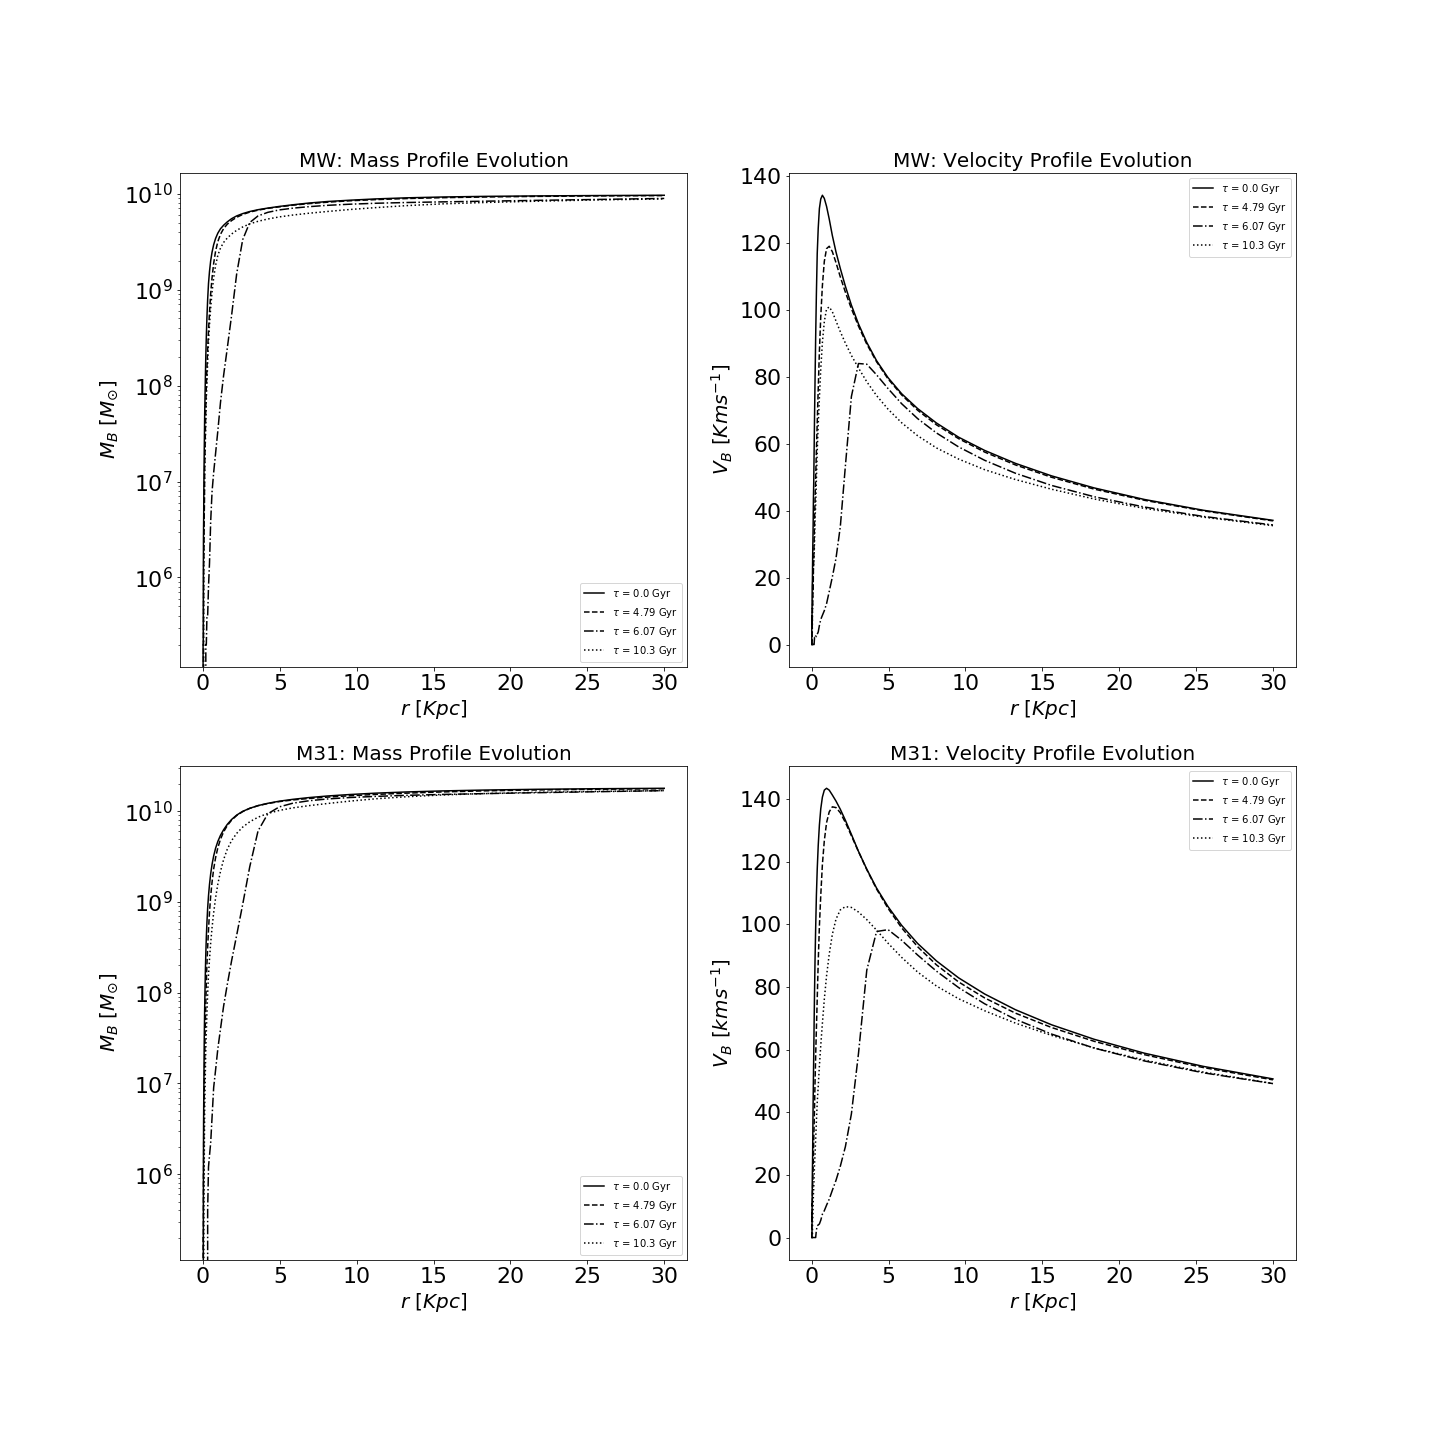
\includegraphics[width=\columnwidth]{MassVelProfile.png}
  \caption{Left column shows Mass Profiles and right columns shows Velocity Profiles at four distinct times that occur at before the merger, post first interaction, post second interaction, and Remnant}
\end{figure}

After the merger takes place at $\tau = 10.3$ Gyr, both MW and M31 particles were examine separately to identify their respective final configurations and how each galaxy contributes to the remnant, see Figure 2. We find that the remnant particles mass distribution becomes localized about the center where the final remnant state is similar that the initial states of both galaxies but with a total mass of $2.9\times 10^{10}M_{\odot}$

\begin{figure}[h]
  \centering
  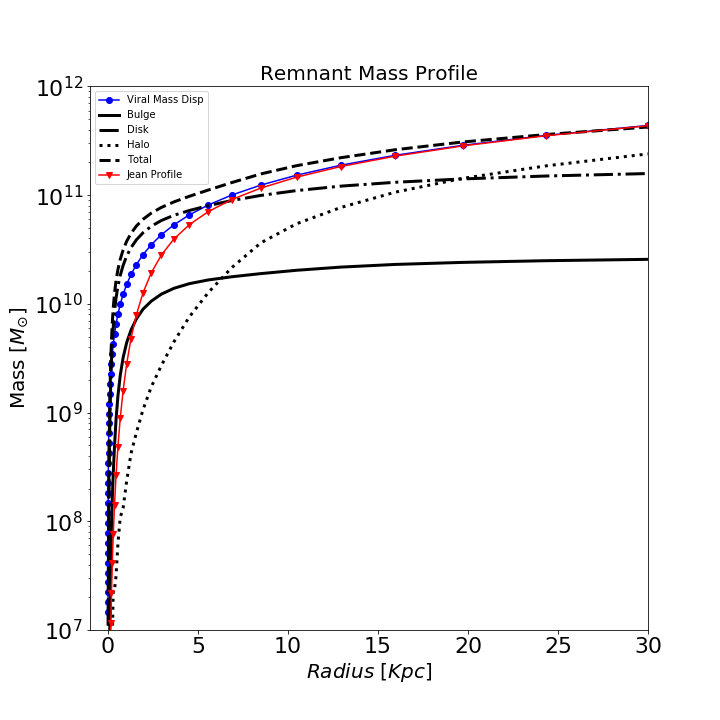
\includegraphics[width=\columnwidth]{RemnantVirial.png}
  \caption{This plot show the Mass Profile all of the components along side the $Virial$ and $Jean's Profiles$, where the Bulge components is represented as the solid line.}
\end{figure}

\begin{figure}[h]
  \centering
  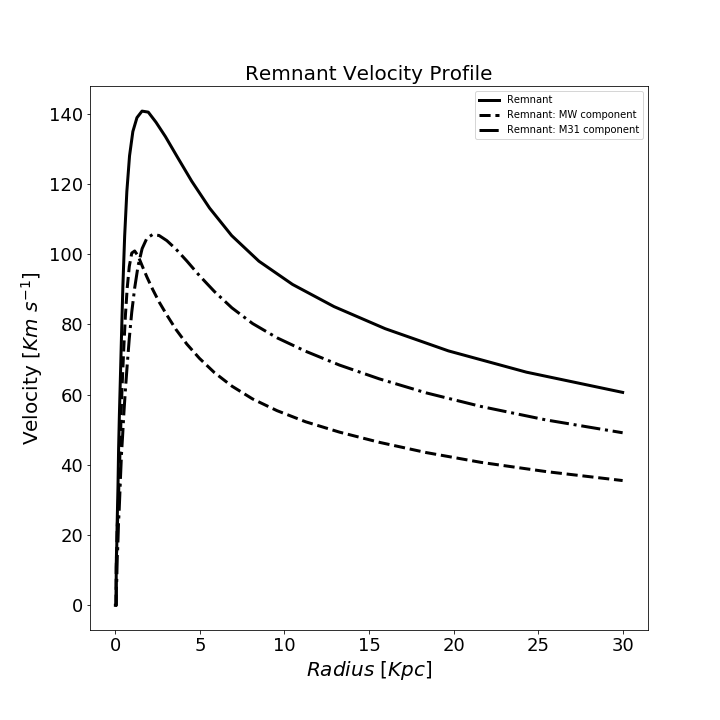
\includegraphics[width=\columnwidth]{RemnantVelProvfile.png}
  \caption{Remnant Velocity Profile along with the individual contribution of MW and M31 particles of bulge component.}
\end{figure}

\subsection{Sersic Profile}
A sersic profile fitting was done on the Remnant to identify whether the bulge resemble a classical or pseudo-bulge, following the equation \begin{equation}
I(r)= I_{0}exp[A(\frac{r}{r_{0}})^{-n}-B]
\end{equation} where $I_{0}$, $A$, $B$, and $n$ are free parameters, and $r_{0}$ is taken to be the effective radius $R_{eff}$ (Half Light Radius) and $I_{0}$ is the central intensity that corresponds to come mass-to-light ration $M/L$. 

An attempt to use $Emcee$ to find the best fitting was used but failed when trying to constraint Sersic index $n$, returning values of $n\geq15$, and $M/L=5$. These values were ignore and proposed to have no significance fundamentally.From this failed attempt it resulted in fitting to be done by hand. The table below shows that values that we find that best fit the data to a Sersic Profile assuming spherical symmetry(Also see figure 3).
  \begin{center}
    \begin{tabular}{ c  c  }
      \hline
      \hline
      Parameter & Value  \\ 
      \hline
      $I_{0}$ & $1.23 \times 10^{8}L_{\odot}$  \\ 
      $R_{eff}$ & 2.17 [kpc] \\
      $A$ & 7.9  \\
      $B$ & 1  \\
      $n$ & 4	 \\
      $M/L$ & 2.2 \\ 
      \hline
    \end{tabular}
  \end{center}
During the fititng process it was seen that the parameter $B$ remained constant. Sersic Profile where $B\neq1$ resulted in a bad fit. The M/L value of 2.2 was chosen based of the results found of William Lake. 
  \begin{figure}[h]
    \centering
    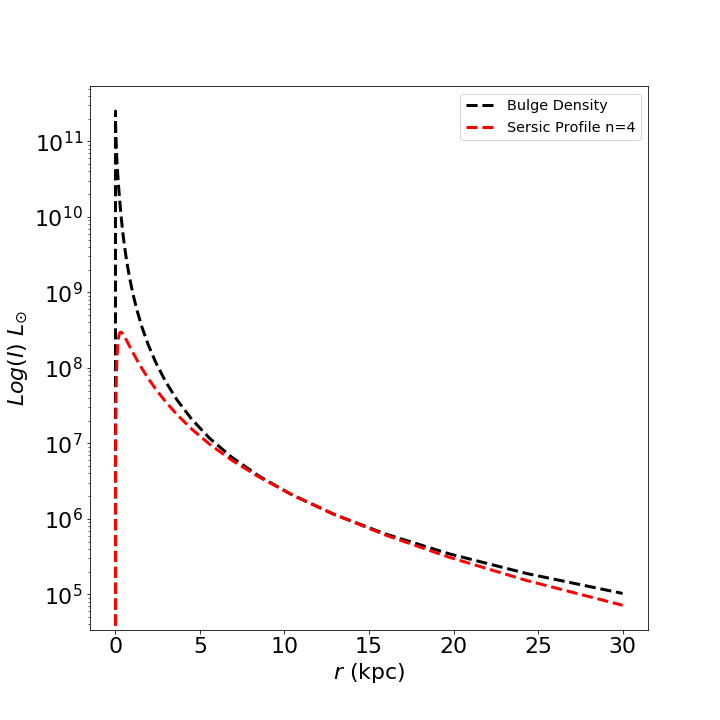
\includegraphics[width=\columnwidth]{sersic.png}
    \caption{Surface Brightness Profile of MW-M31 Remnant with a fitted Sersic Profile of $n=4$}
  \end{figure}

\subsection{Virial Stability}
While two galaxies undergo a merging process it is worth mentioning whether or not the remnant of the two show dynamic stability, suggesting that the newly formed system satisfies the viral theorem. Form general principle the viral theorem is as follow
  \begin{equation}
  2KE = U
  \end{equation}

  \begin{equation}
  M_{viral}(r)=f\frac{rv(r)}{G} = f\frac{r\sigma}{G}
  \end{equation}
where $f$ is some scale factor and $\sigma$ is the velocity dispersion of the system. The Remnant's bulge component does support dispersion where we find the dispersion using the median value rather than the mean to compute the velocity disperion $\sigma=111.72$ km s$^{-1}$. A a scale factor $f=5$ is found that fit a virial profile eq. (3) to our data. 

  \begin{figure}[h]
    \centering
    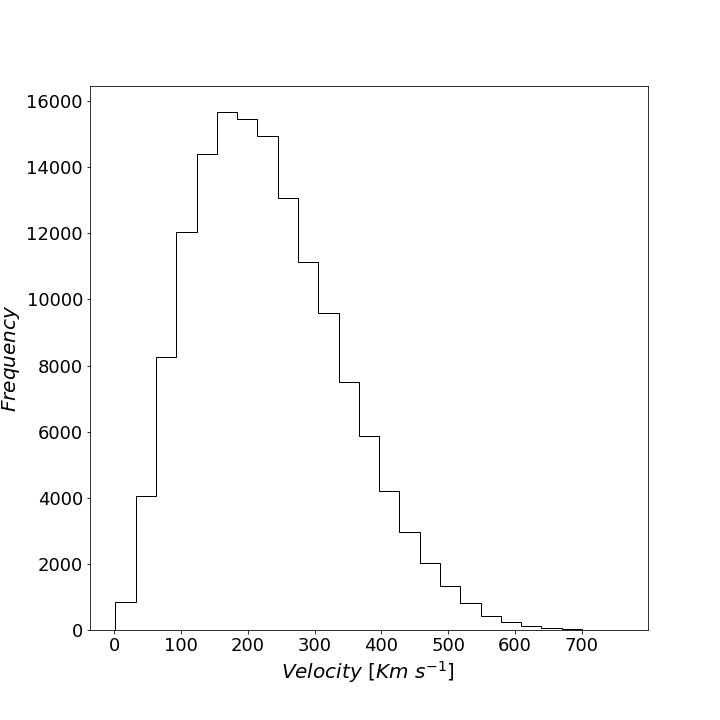
\includegraphics[width=\columnwidth]{dispersion.png}
    \caption{Skewed guassian velocity distribution of the renmant's bulge}
  \end{figure}
  
We also adopted Jeans equation from \citep{walker2009universal} to use to compare our results (see figure 2).
	
    \begin{equation}
	M(r)=\frac{5r_{half}\sigma^{2}(\frac{r}{r_{half}})^{3}}{G[1+(\frac{r}{r_{half}})^{2}]}
	\end{equation}
    
We find that system is dynamic stable in the otter regions and supports the Viral and Jean's Equation. Although our data suggest that there is an excess of mass in the inner most regions. This may suggest that at radii $<10$ kpc may suggest that it may support chaotic motions and has yet to settle into a stable state. A further analysis is required to explain why this occurs and what is actually happening.

\section{Discussion}
Before the formation of the Remnant, the bulge component of both galaxies are perturb by their first fly, resulting in the systems to unbind from their initial states becoming unstable. During their second encounter we identified an altered structure to their mass and velocity profiles, where we assume that the particle near the center are being strongly distorted by both galaxies center of mass as they begin to merge. Once the two merge and the remnant is formed the Remnant's mass and velocity profile look identical to MW and M31 profiles before the merger. The Bulge components of both galaxies are alter overtime even though the no drastic changes occur in both the morphology and the overall dynamics of the system. This suggest that even though particles contained in the bulge are more gravitationally bounded by their systems, will least likely develop significant changes compared to the disk and halo particles, which are more susceptible to decoupling from their system and exchanged particles between colliding galaxies.

Following a Sersic Index found to be $n=4$ indicates that the bulge of the Remnant follows the brightness profile of that of an elliptical galaxy, and contains a classical bulge. Visual inspection was done and found that the shape have elliptical symmetry and found to be dispersion supported.	

\section{Conclusion}
In this paper we find that the remnant of the MW-M31 system contains a classical bulge that is supported dispersion indicated by the Sersic index. Both the bulge component follow similar trends through out the merger process where M31 displays a higher deviation of broaden in both mass and velocity profiles. This implies that some other mechanism causes M31 to be effected more than the MW. Lastly the renmant is found to satisfy the virial theorem, supported by two different profiles. 


\subsection{Future Direction}
A adequate study on the morphology of the bulge component of the MW-M31 remnant should be pursued to determine whether bulge growth occurs and how this growth is effected over time. In this study we have neglected any effects from M33 and should take into account that how the remnant is affected the dwarf galaxy as it continues to fall in toward the remnant.





\bibliography{References}
%\begin{thebibliography}{References}

%\end{thebibliography}

\clearpage

%% Use the figure environment and \plotone or \plottwo to include
%% figures and captions in your electronic submission.
%% To embed the sample graphics in
%% the file, uncomment the \plotone, \plottwo, and
%% \includegraphics commands
%%
%% If you need a layout that cannot be achieved with \plotone or
%% \plottwo, you can invoke the graphicx package directly with the
%% \includegraphics command or use \plotfiddle. For more information,
%% please see the tutorial on "Using Electronic Art with AASTeX" in the
%% documentation section at the AASTeX Web site,
%% http://www.journals.uchicago.edu/AAS/AASTeX.
%%
%% The examples below also include sample markup for submission of
%% supplemental electronic materials. As always, be sure to check
%% the instructions to authors for the journal you are submitting to
%% for specific submissions guidelines as they vary from
%% journal to journal.





























\end{document}

%%
%% End of file `sample.tex'.
